\documentclass{comjnl}

\usepackage{amsmath}
\usepackage{graphicx}
\usepackage{epstopdf}


%% These two lines are needed to get the correct paper size
%% in TeX Live 2016
\let\pdfpageheight\paperheight
\let\pdfpagewidth\paperwidth

%\copyrightyear{2009} \vol{00} \issue{0} \DOI{000}

\begin{document}

\title[Modelling Bidders in Sequential Automated Auctions]{Modelling Bidders in Sequential Automated Auctions}
\author{Kumaara Velan}
\affiliation{Intelligent Systems and Networks Group, Department of
Electrical and Electronic Engineering, Imperial College, London
SW7 2BT, UK} \email{kumaara.velan@imperial.ac.uk}

\shortauthors{K. Velan}
 
\received{00 January 2009}
\revised{00 Month 2009}


%\category{C.2}{Computer Communication Networks}{Computer Networks}
%\category{C.4}{Performance of Systems}{Analytical Models}
%\category{G.3}{Stochastic Processes}{Queueing Systems}
%\terms{Internet Technologies, E-Commerce}
\keywords{Automated Auctions; Analytical Models; Autonomic
Systems; Internet Technologies; E-Commerce; Queueing Systems}


\begin{abstract}
Auctions are mechanisms that formalise the rules with which
automated trading schemes can be conducted, and in this paper we
model the interaction of bidder and seller agents in sequential
computerised auctions. We study the outcome of strategies that a
designated ``special bidder'' (SB) may follow in the presence of a
collection of other bidders in an English auction, under the
assumption that the SB can make bids based on its observation of
the ongoing auction as a collective system. In our model, bidding
and sale events are continuous time random processes with discrete
state-space, where the state-space represents the current value of
the most recent bid. We obtain analytical solutions which allow
the evaluation of measures of interest to the SB such as the
probability of winning, the savings with respect to the maximum
payable price in the event of a win, and the expected waiting time
to win. We examine the effects of the SB's time to bid, and study
how its decisions may be selected so as to optimise the SB's
measures of interest.
\end{abstract}

\maketitle

%\section{Introdução}

\subsection{Processo industrial de manufatura}
A Fig. \ref{fig:processo} apresenta uma visão da planta industrial a ser modelada e simulada.
A composição da planta é a seguinte:
\begin{itemize}
    \item Mesa centralizadora com teste de chapa;
    \item 5 robôs manipuladores;
    \item 4 prensas;
    \item Esteira para destinação final das peças;
\end{itemize}

TODO: descrever processo de manufatura

\begin{figure}[H]%
    \centering
    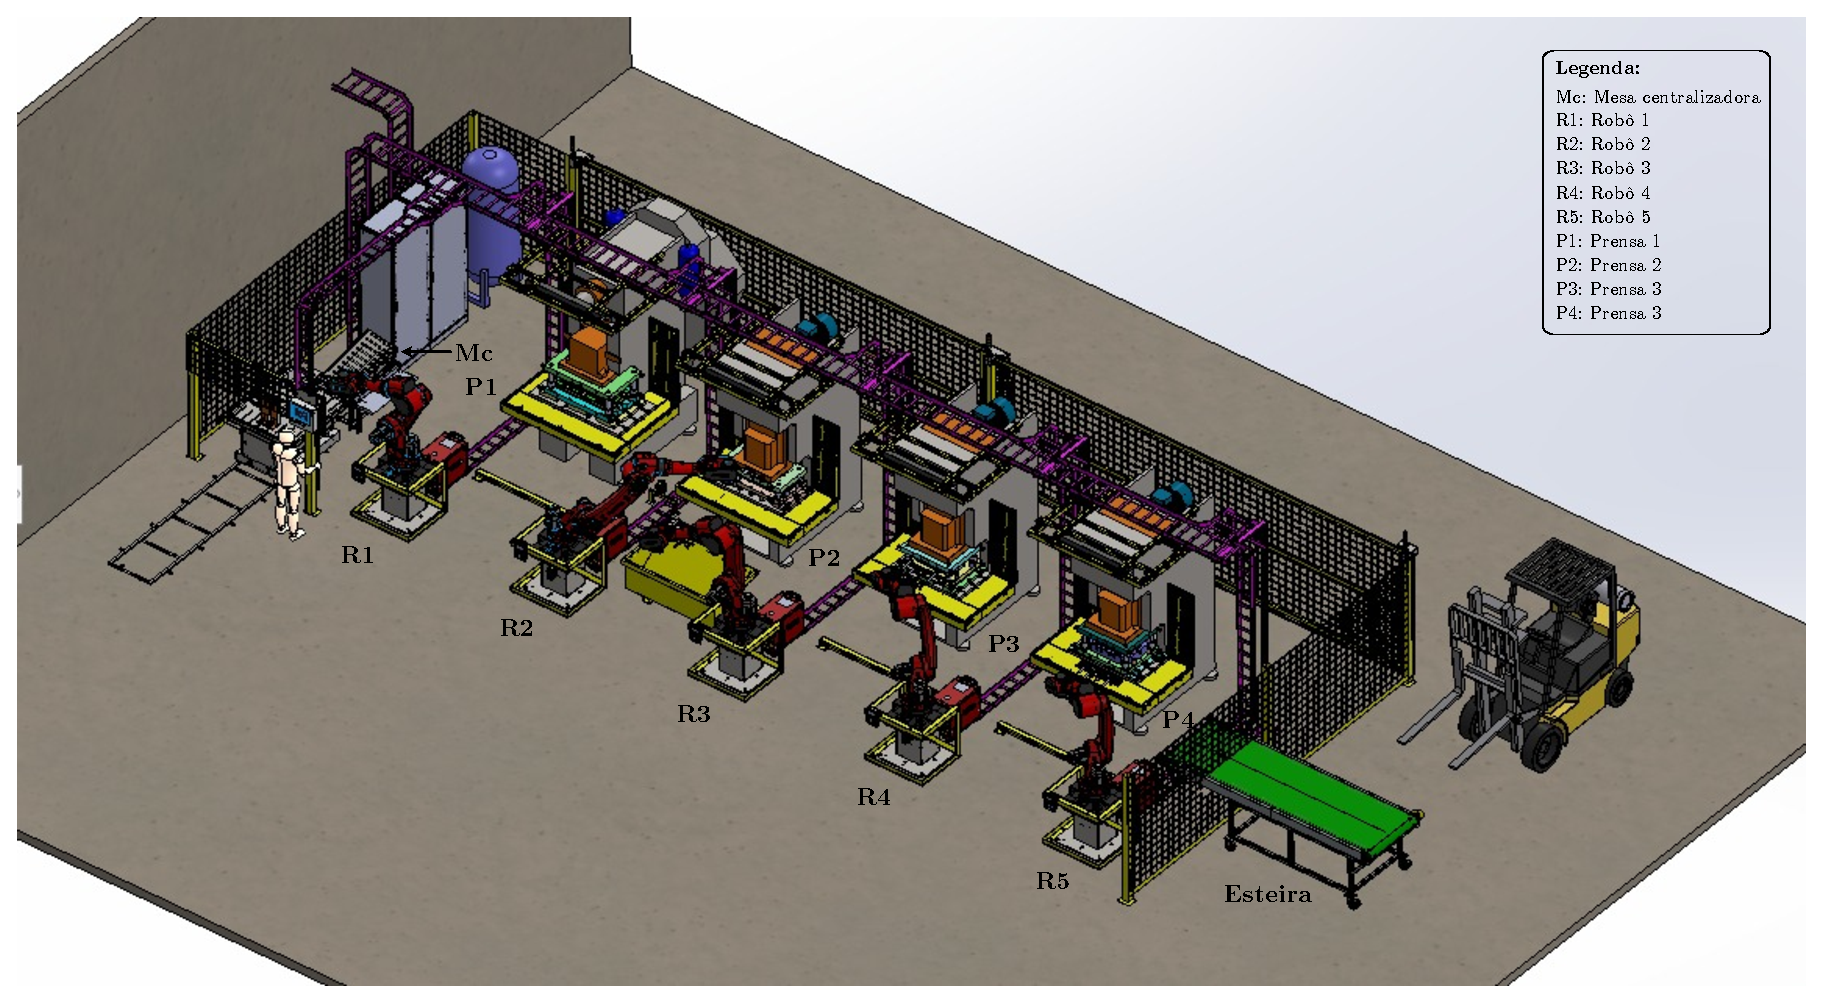
\includegraphics[width=0.8\textwidth]{imagens/processo.eps}
    \caption{Planta industrial}\label{fig:processo}
\end{figure}
%\input{capitulos/revisao_bibliografica.tex}
%\section{Plantas}
Robo 1
\lipsum[1]
\begin{figure}[H]%
    \centering
    \includegraphics[width=0.9\textwidth]{imagens/robo_1.eps}
    \caption{Planta Robo 1}\label{fig:robo1}
\end{figure}

Robo 2
\lipsum[2]
\begin{figure}[H]%
    \centering
    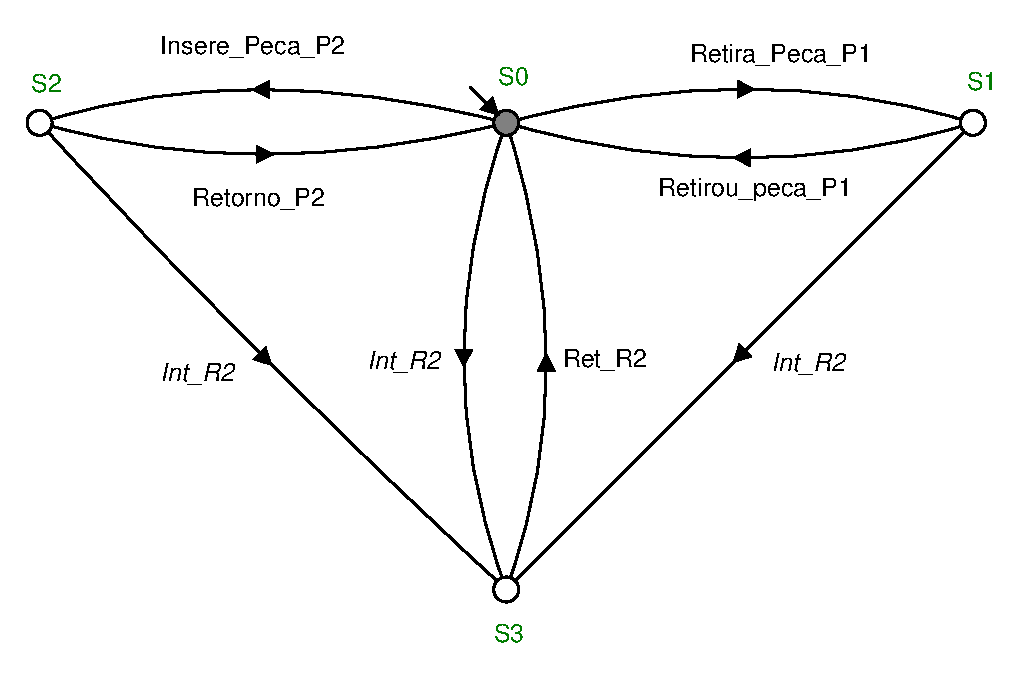
\includegraphics[width=0.9\textwidth]{imagens/robo_2.eps}
    \caption{Planta Robo 2}\label{fig:robo2}
\end{figure}

Robo 3
\lipsum[3]
\begin{figure}[H]%
    \centering
    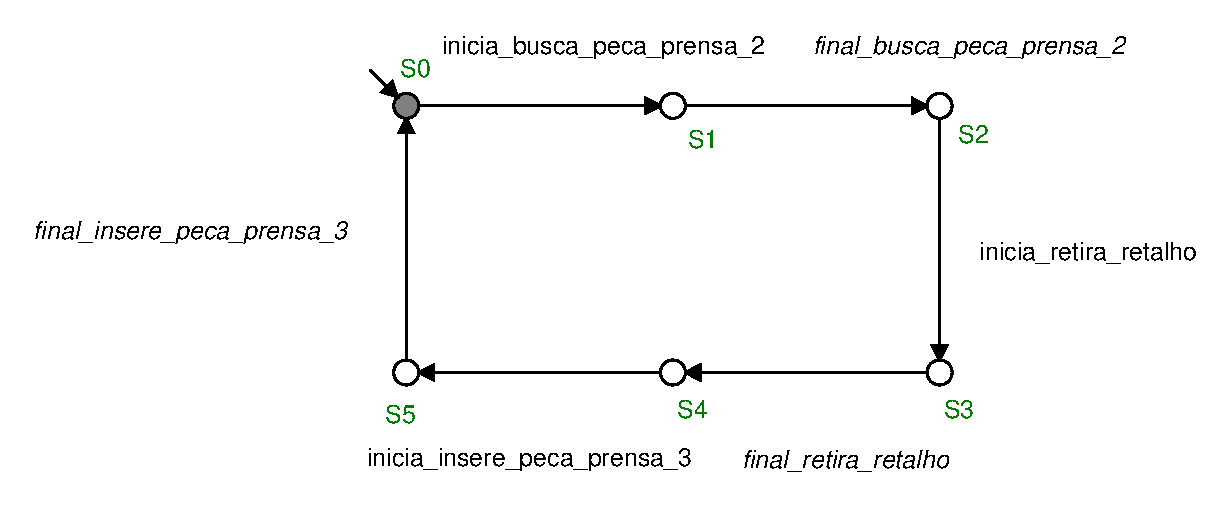
\includegraphics[width=0.9\textwidth]{imagens/robo_3.eps}
    \caption{Planta Robo 3}\label{fig:robo3}
\end{figure}

Robo 4
\lipsum[4]
\begin{figure}[H]%
    \centering
    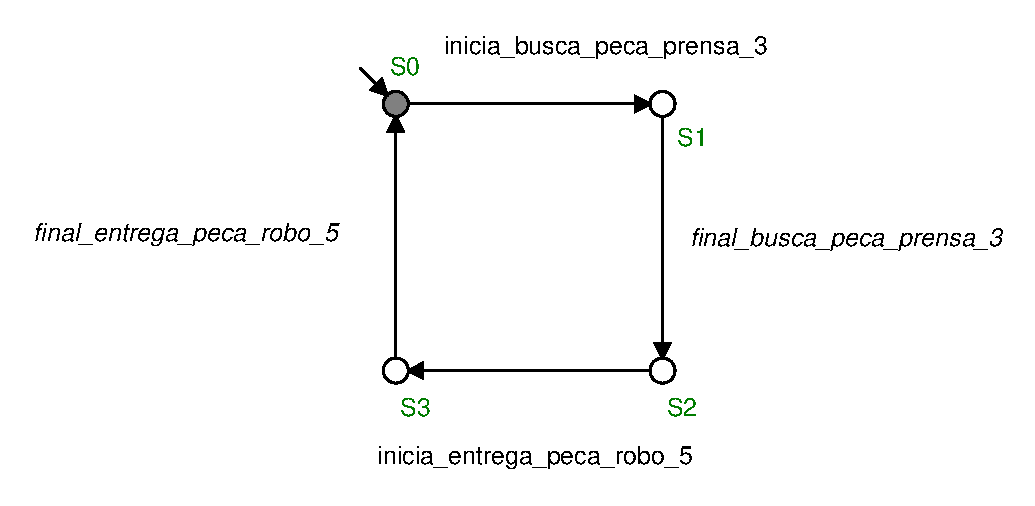
\includegraphics[width=0.9\textwidth]{imagens/robo_4.eps}
    \caption{Planta Robo 4}\label{fig:robo4}
\end{figure}

Robo 5
\lipsum[5]
\begin{figure}[H]%
    \centering
    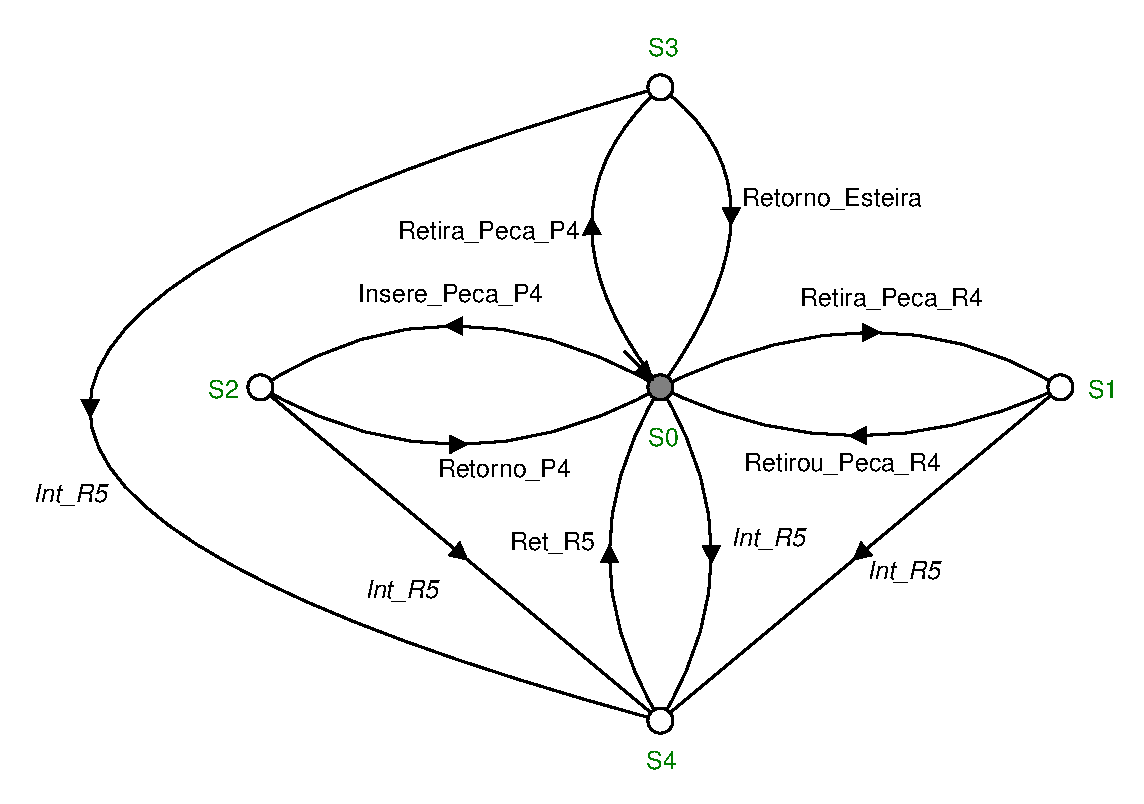
\includegraphics[width=0.9\textwidth]{imagens/robo_5.eps}
    \caption{Planta Robo 5}\label{fig:robo5}
\end{figure}

\lipsum[6]

Citação \cite{bib1} 123 456

\lipsum[7]

\section{Especificações}
\lipsum[1]
\begin{figure}[H]%
    \centering
    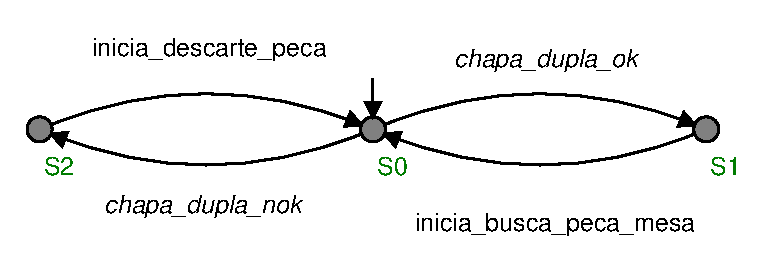
\includegraphics[width=0.9\textwidth]{imagens/E1_robo_1_chapa_dupla.eps}
    \caption{Planta Robo 5}\label{fig:robo5}
\end{figure}

%\section{Conclusões}
TODO: explicar explosão do número de estados do modelo.

\input{capitulos/exemplos.tex}

\nocite{*}

\bibliographystyle{compj}
\bibliography{bibliografia}


\end{document}